\documentclass[10pt]{beamer}
\usepackage[T1]{fontenc}
\usepackage{xeCJK}
\usepackage{listings}
\usepackage{xcolor}
\usepackage{algorithm}
\usepackage{algorithmic}
\usepackage{float}
\usepackage{amsmath,amsfonts,amsthm,bm} % Math packages
\usepackage{multirow}

\definecolor{mygreen}{rgb}{0,0.6,0}
\definecolor{mygray}{rgb}{0.5,0.5,0.5}
\definecolor{mymauve}{rgb}{0.58,0,0.82}
\lstset{ %
	backgroundcolor=\color{white},   % choose the background color
	basicstyle=\footnotesize\rmfamily,     % size of fonts used for the code
	columns=fullflexible,
	breaklines=true,                 % automatic line breaking only at whitespace
	captionpos=b,                    % sets the caption-position to bottom
	tabsize=4,
	commentstyle=\color{mygreen},    % comment style
	escapeinside={\%*}{*)},          % if you want to add LaTeX within your code
	keywordstyle=\color{blue},       % keyword style
	stringstyle=\color{mymauve}\ttfamily,     % string literal style
	numbers=left, 
%	frame=single,
	rulesepcolor=\color{red!20!green!20!blue!20},
  % identifierstyle=\color{red},
  language=c
}

\usetheme{Madrid}

\title{Hello World}
\subtitle[short subtitle]{long subtitle}
\author[Xiangyun Ding]{Xiangyun Ding}
% \institute[UCR]{ucucr}
% \date{March 1, 2020}
\date{\today}

% \small \tiny \large \huge 以及大写的

\AtBeginSection[]
{
	\begin{frame}<beamer>
	  \frametitle{\textbf{Table of Contents}}
	  \tableofcontents[currentsection]
  \end{frame}
}

\begin{document}

\frame{\titlepage}

\section[Table of Contents]{}   %目录
\begin{frame}{Table of Contents}
\tableofcontents
\end{frame}

\section{section1}

\begin{frame}{A sample slide}

  \href{http://v.youku.com/}{a hyperlink} 

A displayed formula:
\[
  \int_{-\infty}^\infty e^{-x^2}dx = \sqrt{\pi}
\]
An itemized list:

\begin{itemize}
  \item itemized item 1, hahaha
  \item itemized item 2
\end{itemize}
\begin{enumerate}
  \item The first item
  \item The second item
\end{enumerate}

\end{frame}

\begin{frame}

\begin{theorem}{1.1}
  In a right triangle, \small{the square of hypotenuse equals
  the sum of squares of two} other sides.
\end{theorem}

\begin{block}{123}
  hello
\end{block}

\begin{description}
  \item[First Item] Description of first item
  \vspace{0.5cm}  %空一行 
  \item[Second Item] Description of second item
\end{description}

\begin{columns}
  \column{.50\textwidth}
  First column text and/or code
  \column{.50\textwidth}
  Second column text and/or code
\end{columns}

\end{frame}

\section{section2}

\begin{frame}{a table}

  \begin{table}[ht]
    \centering
  \fontsize{7.5pt}{11pt}\selectfont{
      \begin{tabular}{ccccccccccc}
        \hline
        \multirow{2}{*}{Matrix} &
              \multicolumn{2}{c}{\texttt{randQB\_EI}(Alg. 2)} & & \multicolumn{2}{c}{\texttt{svds}}& &\multicolumn{4}{c}{Adaptive PCA Framework} \\
              \cline{2-3}
              \cline{5-6}
              \cline{8-11}
              & time (s) & $k$ & & time (s) & $k^*$ & & time (s) & $k$ & Sp1 & Sp2\\
        \hline
        MovieLens-1M&3.83&118& &3.0&117& &{\bf 1.75}&118 & 1.8 & 1.7\\
        hetrec2011&40.3&328& &71.8&325& &{\bf 29.1}&327 & 1.4 & 2.5\\
        BookCrossing&2739&3012& &6758&3004& &{\bf 1004}&3014 & {\bf 2.8} & {\bf 6.7}\\
        MovieLens-20M&1476&883& &3722&879& &{\bf 704}&883 & 2.1 & 5.3\\
        \hline
      \end{tabular}
  }
  
  \end{table}

\end{frame}

\begin{frame}

  \begin{figure}[tb]
    \label{fig:figure1}
    \centering
    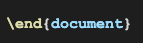
\includegraphics[width=0.5\textwidth]{t1.png}
    \caption{Caption here}
  \end{figure}

\end{frame}

\begin{frame}{a code}

  \lstinputlisting[lastline=30,
language=Python,
frame=single,
label=python]
{temp.py}

\end{frame}

\begin{frame}{an algorithm}
  

  \begin{algorithm}[H]
    \algsetup{linenosize=\tiny} \scriptsize
  \begin{algorithmic}[1] %一行一个标行号
    \REQUIRE $\mathbf{A}\in\mathbb{R}^{m\times n}$~$(m \le n)$, block size $b$, pass parameter $q > 2$
    \ENSURE $\mathbf{U}\in\mathbb{R}^{m\times k}$, $\mathbf{S}\in\mathbb{R}^k$, $\mathbf{V}\in\mathbb{R}^{k\times n}$ for certain accuracy criterion
%    \STATE $E=\left\|\mathbf{A}\right\|^2; ~ thresh=\varepsilon^2\times E$
      \STATE $\mathbf{Q} = [~ ]$, ~ $\mathbf{B} = [~ ]$
      \FOR {$l=1, 2, 3, \cdots$, }
      \STATE \textbf{if} $q$ is an even number
        \STATE \quad\quad$\bm{\Omega}=$ randn($n,b$),$\mathbf{Y}=\mathbf{A}\bm{\Omega}-\mathbf{Q}(\mathbf{B}\bm{\Omega})$
        \STATE \quad\quad$[\mathbf{Q}_l, ~ \sim]=$lu($\mathbf{Y}$) \quad \quad \quad \quad \quad \quad \# LU factorization replaces QR factorization
      \STATE \textbf{else} 
        \STATE \quad\quad$\mathbf{Q}_l=$randn($m,b$) \quad \quad \quad \quad \quad \quad \# when $q$ is an odd number
      \FOR {$t=1,2,\cdots,\lfloor\frac{q-1}{2}\rfloor$}
        \STATE \textbf{if} $t==\lfloor\frac{q-1}{2}\rfloor$
          \STATE \quad\quad$\mathbf{R}=\mathbf{A}^\mathrm{T}\mathbf{Q}_l$ \quad \quad \quad \quad \quad \quad \quad \# remove one orthogonalization 
          \STATE \quad\quad$\mathbf{Q}_l= \mathrm{orth}(\mathbf{A}\mathbf{R}-\mathbf{Q}(\mathbf{B}\mathbf{R}))$ \quad \quad \# the last one in power iteration 
        \STATE \textbf{else}
          \STATE \quad\quad$[\mathbf{Q}_l, \sim] =$lu($\mathbf{A}(\mathbf{A}^\mathrm{T}\mathbf{Q}_l)$) \quad \quad \# LU factorization replaces QR factorization
      \ENDFOR
      \STATE $\mathbf{Q}_l = \mathrm{orth}(\mathbf{Q}_l-\mathbf{Q}(\mathbf{Q}^\mathrm{T}\mathbf{Q}_l)),\mathbf{B}_l=\mathbf{Q}_l^\mathrm{T}\mathbf{A}$
      \STATE $\mathbf{Q}=\begin{bmatrix}\mathbf{Q}&\mathbf{Q}_l\end{bmatrix}, ~ \mathbf{B}=\begin{bmatrix}\mathbf{B}\\\mathbf{B}_l\end{bmatrix}$
%      \IF {$E-\left\|\mathbf{B}_i\right\|^2<thresh$}
%        \FOR {$j=1,2,\cdots,b$}
%          \STATE $E = E - \left\|\mathbf{B}_{i}(j,:)\right\|^2$
%          \STATE if $E<thresh$ then break
%        \ENDFOR
%        \STATE break
%      \ENDIF
%      \STATE $E=E-\left\|\mathbf{B}_i\right\|^2$
    \STATE \textbf{if} {termination criterion is met}
    \STATE \quad\quad$k$ is determined and then break
    \ENDFOR
%  \STATE $k=b\cdot i+j$
  \STATE $[\mathbf{\hat{U}},\mathbf{\hat{S}},\mathbf{\hat{V}}] = \mathrm{eigSVD}(\mathbf{B^\mathrm{T}})$ \quad \quad \quad \quad \# use eigen-decomposition to compute SVD
%  \STATE $\mathbf{U}=\mathbf{Q}\mathbf{\hat{U}}(:, 1:k); ~ \mathbf{S}=\mathbf{\hat{S}}(1:k); ~ \mathbf{V}=\mathbf{\hat{V}}(:, 1:k)$
    \STATE $ind=lb:-1:lb-k+1$
  \STATE $\mathbf{U}=\mathbf{Q}\mathbf{\hat{V}}(:, ind),  ~ \mathbf{S}=\mathbf{\hat{S}}(ind), ~ \mathbf{V}=\mathbf{\hat{U}}(:, ind)$
	\end{algorithmic}
\end{algorithm}

\end{frame}

\section{section3}
\begin{frame}{hihi}
  \begin{itemize}
    \item<1-> First point, shown on all slides.
    \item<2-> Second point, shown on slide 2 and later.
    \item<3-> Third point, also shown on slide 2 and later.
    \item<4-> Fourth point, shown on slide 3.
  \end{itemize}
\end{frame}

\begin{frame}
  \hspace{3cm}
  \Huge{Questions?}
\end{frame}

\end{document}